% document formatting
\documentclass[10pt]{article}
\usepackage[utf8]{inputenc}
\usepackage[left=1in,right=1in,top=1in,bottom=1in]{geometry}
\usepackage[T1]{fontenc}
\usepackage{xcolor}

% math symbols, etc.
\usepackage{amsmath, amsfonts, amssymb, amsthm}

% lists
\usepackage{enumerate}

% images
\usepackage{graphicx} % for images

% code blocks
\usepackage{minted, listings} 

\graphicspath{{./assets/images/Week 2}}

\newcommand{\solution}{\textbf{Solution:}} 

\title{CHEM 20B Week 2}

\author{Aidan Jan}
\date{\today}

\begin{document}
\maketitle
\section*{States of Matter}
The fundamental difference between states of matter is the distance between particles.
\begin{center}
    \includegraphics*[scale=0.5]{W2_1.png}
\end{center}

\section*{Molar Volume}
\[V_m = \frac{V}{n}\]
\begin{itemize}
    \item For 1 mole of solid or liquids $V_m = 10 \sim 100$ cm$^3$ at room conditions
    \item For 1 mole of gas, $V_m \approx 24000$ cm$^3$ at room conditions
\end{itemize}

\section*{Compressibility}
$\kappa$ (kappa) = fractional change in volume per pressure change, when T is fixed.
\[\kappa = -\frac{1}{V} \left(\frac{\partial V}{\partial P}\right)_T\]
\[\kappa = -\frac{1}{V} \left(\frac{\Delta V}{\Delta P}\right)\]
$\kappa$ (Gases) is large.
$\kappa$ (Solids/Liquids) $\sim 10^{-4}$/atm, much smaller than for gases.

\section*{Thermal Expansion}
The thermal expansion coefficient measures the percent change in volume when we raise the temperatrue.  $\alpha$ (alpha) = fractional change in volume / temperature change.
\[\alpha = \frac{1}{V} \left(\frac{\partial V}{\partial T}\right)_P\]
\[\alpha = \frac{1}{V} \left(\frac{\Delta V}{\Delta T}\right)\]

\section*{Intermolecular Forces}
\begin{center}
    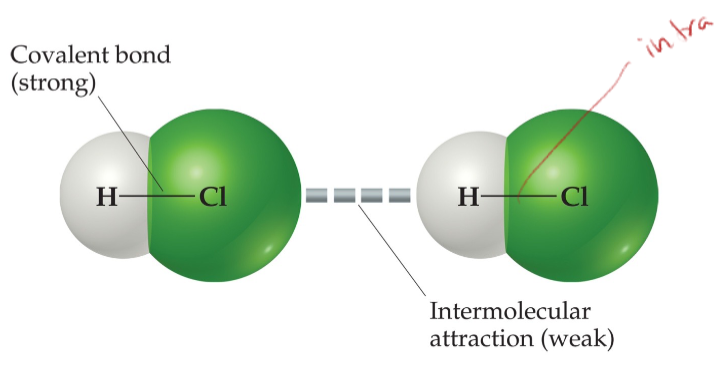
\includegraphics[scale=0.5]{W2_2.png}
\end{center}
The attractions between molecules are not nearly as strong as the intramolecular attractions that hold compounds together.\\\\
They are, however, strong enough to control physical properties such as boiling and melting points, vapor pressures, and viscosities.
\begin{center}
    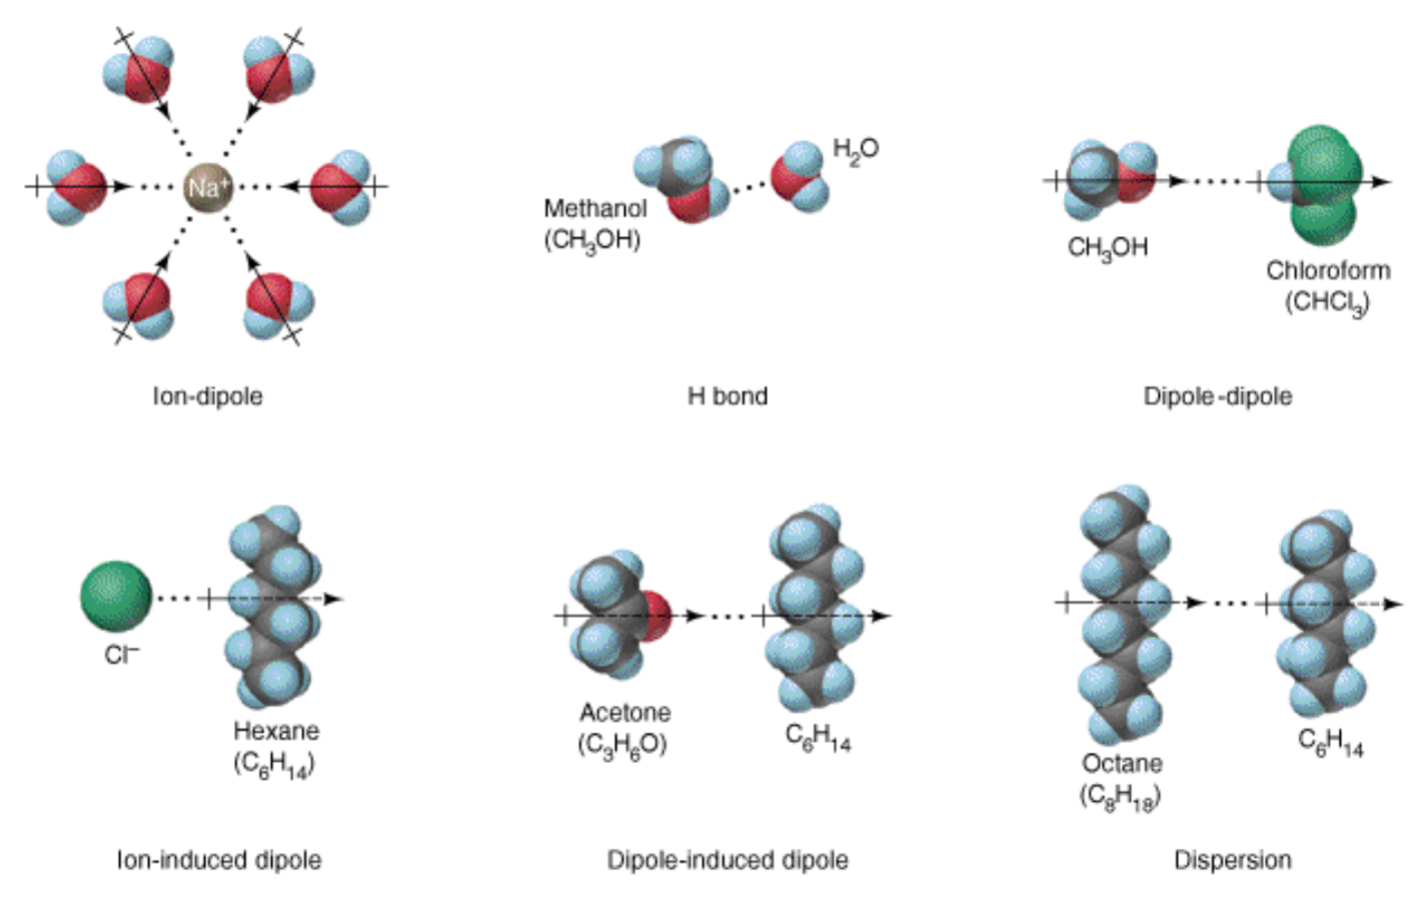
\includegraphics[scale=0.3]{W2_3.png}
\end{center}
\textbf{Types of Intermolecular Forces}
\begin{itemize}
    \item Ion-Ion Forces
    \item Dipole-Dipole Forces
    \item Ion-Dipole Forces
    \item Charged-Induced Dipole Forces: Polarizability
    \item Induced Dipole - Induced Dipole Forces: London Dispersion Forces
    \item Repulsive Forces
\end{itemize}

\subsection*{Ion-Ion Forces}
\begin{itemize}
    \item \"Columbic\", i.e., due to attraction between opposite charges
    \item Long range $\sim$ 1/R
    \item Not directional (does not depend on relative orientation, each ion interacts equally strongly with neighboring ions on all sides)
    \item Strong (the same strength as covalent interactions)
    \item Example: NaCl
    \begin{center}
        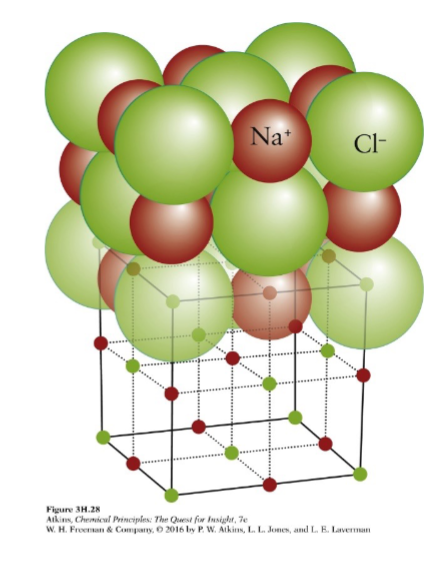
\includegraphics[scale=0.5]{W2_4.png}
    \end{center}
\end{itemize}

\subsection*{Ion-Dipole Forces}
\begin{itemize}
    \item Act between ions and molecules with permanent dipole moments.
    \item Stronger than dipole-dipole, weaker than ionic
    \item Long range $\sim 1/R^2$
    \item Directional (a rotation of the dipole by 180 degrees turns the interaction from attractive to repulsive, or vice versa).
    \item Example: Water being attracted to ions
    \begin{center}
        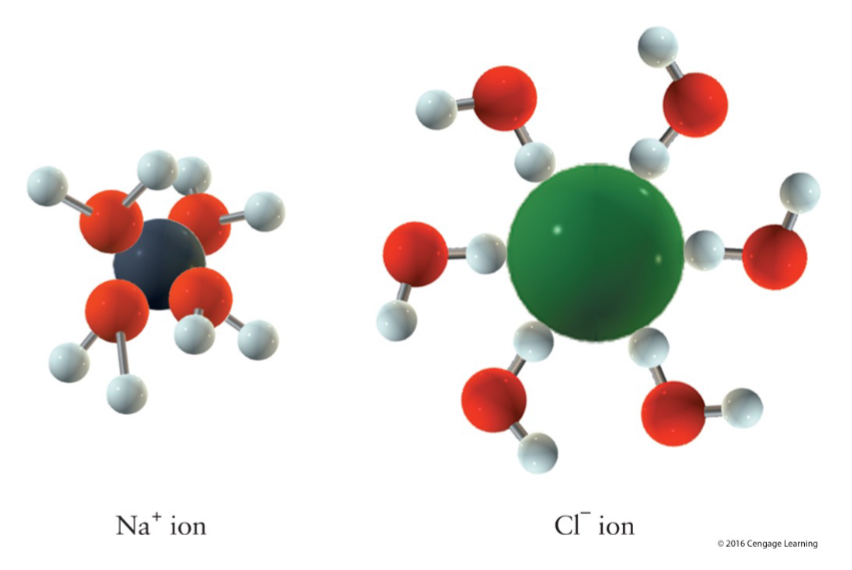
\includegraphics[scale=0.5]{W2_5.png}
    \end{center}
\end{itemize}

\subsection*{Dipole-Dipole Forces}
\begin{itemize}
    \item The dominant force between polar molecules.
    \item Long range $\sim 1/R^3$ but not as long-range as ion-ion or ion-dipole
    \item Relatively strong: $\sim$ 5-50 kJ/mol
    \item Directional
    \item Example: HCl molecules aligning in opposite directions
    \begin{center}
        \begin{align*}
            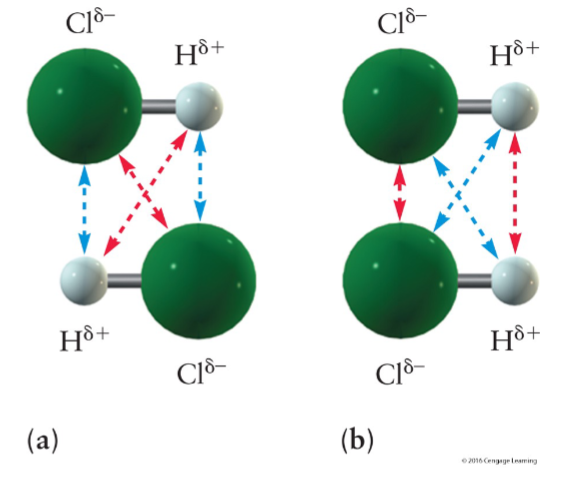
\includegraphics[scale=0.5]{W2_6.png}
            \hspace{2cm}
            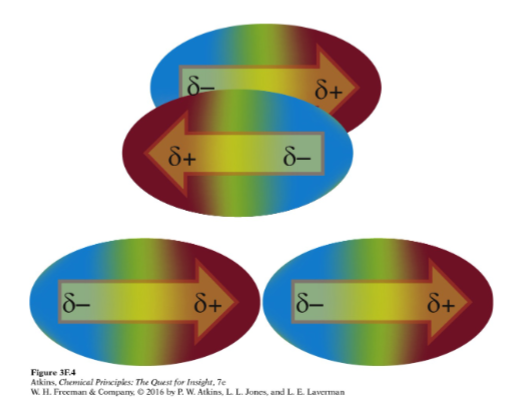
\includegraphics[scale=0.5]{W2_7.png}
        \end{align*}
    \end{center}
\end{itemize}

\subsection*{Charge-Induced Dipole Forces: Polarizability}
\begin{itemize}
    \item The electrons in a nonpolar molecule are distributed symmetrically, the distribution can be distorted by an approaching electrical charge.
    \item Na$^+$ induces a temporary dipole moment in the Ar atom
    \item The electron distribution of the nonpolar molecule is said to be polarizable
    \item Weak
    \item Short range
    \begin{center}
        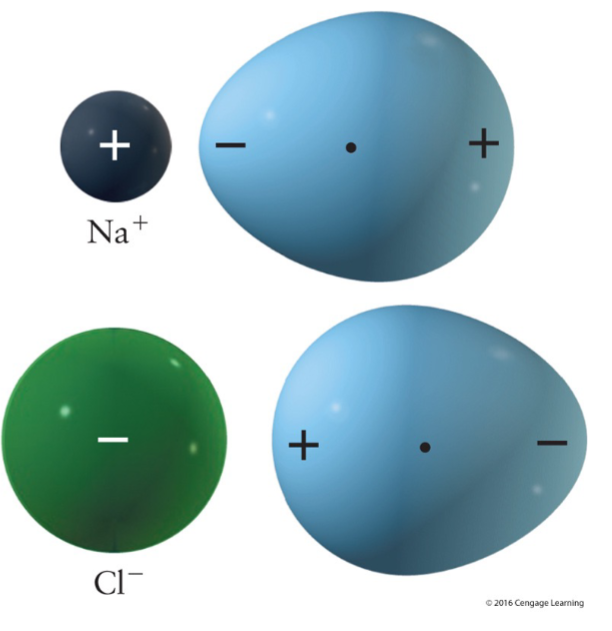
\includegraphics[scale=0.5]{W2_8.png}
    \end{center}
\end{itemize}

\subsection*{Induced Dipole - Induced Dipole Forces: London Dispersion Forces}
\begin{itemize}
    \item \textbf{Instantaneous dipole moments} create distortions in the electron cloud, which become partially positively ($\delta^+$) and partially negatively ($\delta^-$) charged.
    \item Always attractive
    \item It is not very directional (i.e., even for molecules, the interaction does not depend much on the relative orientation of the molecule).
    \item Very short-range, $1/R^6$
    \item Since always attractive, adds up.  Can be significant for large surfaces - causes two regions with large surface area that are placed near each other to stick together.
    \item The only force present for nonpolar molecules
    \begin{center}
        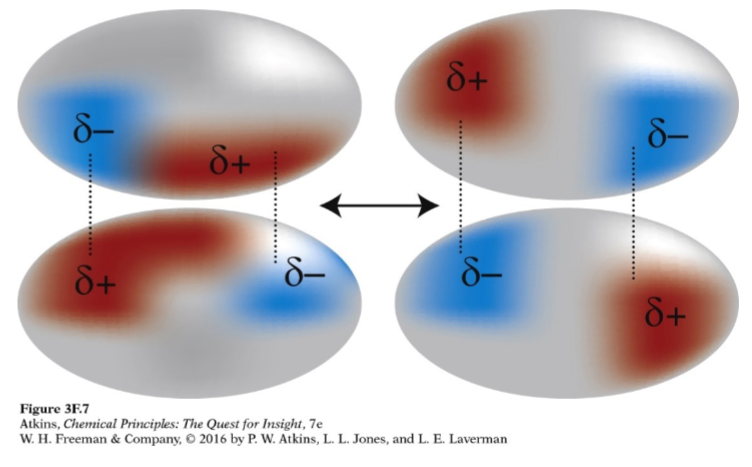
\includegraphics[scale=0.5]{W2_9.png}
    \end{center}
\end{itemize}

\subsubsection*{London Dispersion Forces: Size and Shape}
\begin{itemize}
    \item As size increases (more shells), polarizability increases.  This causes melting and boiling points to increase.
    \item Rod-like molecules have a \textbf{greater surface area}, which allow for \textbf{more contact points} for molecules to join togerther.
    \item Ball or spherical shaped molecules have \textbf{fewer contact points} for molecules to join together.
    \begin{center}
        \begin{align*}
            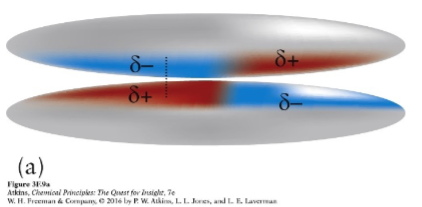
\includegraphics[scale=0.7]{W2_10.png}
            \hspace{1.5cm}
            \includegraphics*[scale=0.7]{W2_11.png}
        \end{align*}
        \includegraphics*[scale=0.5]{W2_12.png}
    \end{center}
\end{itemize}

Continued in Week 3...

\end{document}